% !TEX root =  ../thesis.tex

Before being able to understand how profiles change in time and find anomalous profiles and transactions, we need to understand how a profile is defined and computed.

After preliminary definitions and an explanation of the different types of profiles, we will focus more on their mathematical representation (the histogram) and its properties, with the objective of defining a distance function able to satisfy our requirements.

\section{Definition of User Profile}

In order to define a User Profile, we will first introduce a few preliminary definitions.

\begin{description}
  \item[user] a single client of the bank, be it a private or a company, identified by a unique code in the dataset.
  \item[feature] a dimension of a transaction, which can be of type Integer, Real or Categorical
  \item[window] a period of time on which transactions are grouped and a profile is defined. For each window, only one profile exists, and vice versa. Windows in this thesis will in general be of one month.
  \item[bin selection] the procedure of mapping a value to a bin in a histogram
\end{description}

A profile is computed from a set of transactions that belong to the same time window, and it is composed of a set of histograms, one for each feature. The sum of each histogram is equal to the total number of transactions. Each histogram is composed of 2 or more bins, where the value of each bin is defined as the number of transactions for which the value of the feature related to the histogram is included in the set of bin values.

\subsection{Histograms and their properties}

Now we shift the focus from the overall user profile to the properties of a single histogram. A single histogram represent a pattern in the user transactions over that feature. For instance, let us take the feature `amount' in consideration. The amount is simply the monetary value of a transaction, expressed in euros. A histogram mostly flat, such as in figure \ref{fig:flat_histogram}, means that the user makes transactions of all amounts indiscriminately. If the histogram is mostly skewed to the left, the user will prefer smaller transactions; if to the right, bigger transactions.

\begin{figure}[h]
\centering
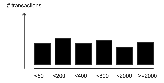
\includegraphics[width=250]{images/flat_histogram.pdf}
\caption{Histogram representing the distribution of transactions over the `amount' feature}
\label{fig:flat_histogram}
\end{figure}

To understand this, only the shape of the histogram is relevant, and can therefore be normalized to have sum one and interpreted as a dicrete probability distribution.

We refer to a histogram with the notation $H$, and to the value of bin $i$ with $H(i)$.

We follow the classification of histograms as proposed in \cite{histogram}, which divides histograms in three families based on their type of measurement:

\begin{description}
\item[ordinal] the values are ordered, such as numbers or more in general anything that can be ordered.
\item[nominal] the values are a finite set of possible categories, without any ordering implied.
\item[modulo] the values are ordered in a `ring' where the rightmost values are close to the leftmost ones, as in the arithmentic modulo operation.
\end{description}

\section{Distance between histograms}

In order to compute how profiles change over time, we need to introduce the concept of a distance between histograms. This topic is central to this thesis, and will be explored in depth, as it provides the basis for the whole temporal profile analysis system.

We refer to the distance between histgrams $H(A)$ and $H(B)$ as $d(H(A), H(B))$.
The distance function will need to be specified over histograms of the same family, and possibly be specialized for each one.

To fullfill the requirements of the temporal analysis, the distance function will have to satisfy a few properties. To better understand why these properties are necessary, an understanding of the system design is useful and can be found in chapter~\ref{design}.

In the following list we will explain which properties it will have to satisfy and why such properties are necessary.
\begin{description}
  \item[reflexive] $d(H(A), H(A)) = 0$. Since with our distance function we will be measuring the variations in spending profiles over time, we have to assign a null variation to a profile that does not change at all.
  \item[commutative] $d(H(A), H(B)) = d(H(B), H(A))$. The necessity for this property is less obvious, because we might want to consider shifts in certain directions as more relevant than in others. However, our design treats all variations in the same way, without giving a meaning to the direction of such variations. For instance, if a user changes her spending profile from mostly low amount transactions to mostly high amount transactions, we want to produce the same distance value as if the shift was reversed. This ensures that our approach remains generic.
  \item[non negative] $d(H(A), H(B)) \geq 0$. Considering that we require our function to be reflexive, and therefore have a $0$ point, having a negative function would mean differentiating distances in 2 directions, such as increase and decrease. As explained in the previous paragraph, we do not want to assign a meaning to the direction of the shift, but only to its magnitude, therefore the function should be non negative.
  \item[positional] for ordinal and modulo histograms, the distance between bins should be taken into account. In other words, the distance function should be a function of the order of the bins, in additions to being a function of their values. Of course, not any relation between the order of the bins and the final distance value is acceptable. Our goal is to reduce the distance when bins with a value $\geq 0$ are close together, since small variations in positions should be considered noise. This property will be discussed in greater details in the following paragraphs.
\end{description}

Before continuing to an analysis of possible distance functions, a quick note on a property that we did not require: \textbf{triangle inequality}. This property says that, for any three histograms $A$, $B$ and $C$, $d(H(A), H(B)) \geq d(H(A), H(C)) + d(H(C), H(B))$.

An example of distance function that does not satisfy this property is the euclidean distance to the power of 2, defined as the sum over each dimension $i$ of $(H(A,i) - H(B,i))^2$. In this case, longer distances will be accounted for in a more than linear fashion. This is not in contrast with our design, as hypothetically it might be possible that such a function resulted in higher performance, accounting more for greater shifts than smaller ones.

Based on a few tests using the euclidean function to the power of $x$, with $x > 1$, we did not find any big difference (positive or negative). In conclusion, we do not require this property and leave experimenting with distance functions that violate it as a possible future work.

\subsection{Positionality: noise and information}

In this section we will delve further in what we mean by positionality and why we think this is essential for our work.
First, let us make an example to better understand:\\
$H(A) = [1, 0, 0, 0, 0]$\\
$H(B) = [0, 1, 0, 0, 0]$\\
$H(C) = [0, 0, 0, 0, 1]$

The desired behavior of our distance function will depend on the type of these histograms:
\begin{description}
  \item[nominal] all distances should be equal
  \item[ordinal] $d(H(A), H(B)) < d(H(A), H(C))$ since the bins containing a 1 are further apart in the second case
  \item[modulo] $d(H(A), H(B)) = d(H(A), H(C))$ since the bins containing a 1 are next to each other, if we see the histogram as a ring
\end{description}

We say that the distance is \textit{shuffling invariant} for nominal histograms and \textit{shuffling dependent} for ordinal and modulo histograms.

We think this property is desirable in our scenario, where a shift in spending habits from transactions around 500 euros to transactions around 800 euros is less relevant than a shift to transactions around 5000 euros.

The issue of positionality can be interpreted in terms of information and noise. Continuing with the amount example, a shift in the order of 100 euros can be interpreted as noise, while a greater shift in the order of thousands of euros conveys real information. We can then formulate our goal in a more high level version: we want our distance function to \underline{consider relevant information and be resiliant to noise in the histogram variations}.

We will now review a few distance functions that can be applied to histograms and finally select the one that better satisfies all the properties we need.

\subsection{Vector representation based distances}

Histograms can be seen as vectors and any distance function that work with vectors can therefore be used. The two easiest distances are:
\begin{description}
  \item[city block] sum over each dimension $i$ of $|H(A,i) - H(B,i)|$
  \item[euclidean] squared sum over each dimension $i$ of $(H(A,i) - H(B,i))^2$
\end{description}

As with all vector based distances, these distances are shuffling invariant and therefore do not satisfy positionality at all. We still included them here because, when complemented with appopriate filtering, they can serve our purpose, as explained in the following paragraphs.

\subsection{Miminum distance of pair assignments}

The MDPA (minimum distance of pair assignments) is a distance function that, at a basic level, satisfies all the properties we require, as shown in \cite{histogram}. To define the MDPA consider two sets of n elements, A and B, which define histograms $H(A)$ and $H(B)$. The MDPA is intuitively equal to the minimum total cost of the `moves' that we need to make in order to transform the first histogram in the second one. A move is defined as subtracting $x$ from bin $i$ and adding it to bin $j$. The cost of a move is $x * d(i, j)$ where $d(i, j)$ is the linear distance between the two bins.

This distance can be used for ordinal and modulo histograms as it takes into account the position of bins. Moreover, efficient algorithms exist for computing the MDPA distance. We have implemented the algorithm for the ordinal type and tested it, as documented in section \ref{sec:mdpa_test}.

However, the problem is that in these algoritms the distance $d(i, j)$ between bins is considered to be a linear distance. We think that this is not optimal in our scenario, since the meaning of such distance depends on the feature measured by the profile associated with the histogram and other distances could be necessary. In particular super-linear distance functions could make more sense in real world situations, where for instance $d(i, j), i=0, j=4$ should be more than double than $d(i, j), i=0, j=2$.

To verify this assumption, we tested the MDPA function and compared it to our approach (as explained in the next section) and found a substantial improvement. Of course, defining a custom distance $d(i, j)$ that is non linear is possible in MDPA, but leads to a generic optimization problem with exponential complexity. Efficiency being a key component of our design, we discarded this direction of research.

\section{Low-pass filtered euclidean distance}

Our approach is based on a completely different technique: instead of finding another distance algorithm that takes bin position into account, we apply a low-pass filter to the histograms and then apply a normal euclidean distance.

In this way we can achieve our goal of reducing noise and taking into account the overall shape of the histogram, which represents the spending pattern of the user, rather than the small variations in each bin. 

The low-pass filter we decided to use is the gaussian filter, which is a very well known filter used to remove high frequency noise, reducing the variance in the values of the histogram.

The two dimensional gaussian smoothing filter, also known as gaussian blur, is often used in computer vision to perform contour and shape detection. In our situation, it solves a similar problem in revealing the shape of the histogram.

\subsection{Gaussian function and Weierstrass transform}

The gaussian function with mean $\mu = 0$ is defined as:
\begin{displaymath}
  \frac{1}{\sigma\sqrt{2\pi}}e^{-\frac{x^2}{2\sigma^2}}
\end{displaymath}

The smoothing filter that results from the convolution of the input histogram with the Gaussian function is the Weierstrass transform.

Using the weierstrass transform, each bin in the smoothed histogram is the weighted average of its surrounding bins, using the gaussian function to compute the weights.

For instance, the weight assigned in the weighted average to a bin next to the one being computed is given by the gaussian function where $x = 1$, being $x$ the distance between the bins. We can consider as insignificant bins with distance $x > 3\sigma$.

This method can account for different types of histograms and can be tuned by adjusting the parameter $\sigma$ of the gaussian function in order to specify how much the histograms should be smoothed before computing their euclidean distance.

In particular, we have as always three types of histograms to account for:

\begin{description}
  \item[nominal] no smoothing should be applied, the euclidean distance can be computed directly
  \item[ordinal] smoothing should be applied, if the weighed average would includes bins outside of the histogram range (for instance, when computing the average for the first or last bin) it should be limited to those available.
  \item[modulo] smoothing should be applied, but in this case when bins are outside of the histogram range they will be taken from the other end of the histogram, following the rules of the arithmentic modulo operator.
\end{description}

\subsection{Preservation of properties}

The euclidean function is reflexive, non-negative and commutative but not positional. We need to prove that, applying the gaussian filter to both input histograms before applying the euclidean distance, we are preserving those properties and in addition satisfying positionality.

\begin{description}
  \item[reflexive] Since the gaussian blur is a deterministic mathematical transform that will always give the same result given the same input, we can state that \\
    $d(F(H(A)), F(H(A))) = 0$.
  \item[commutative] Following the same logic, the transform does not affect commutativity of the euclidean distance.
  \item[non-negative]
    However transformed, the input of the euclidean distance does not affect its non negativity (the difference over each dimension is squared).
  \item[positional] general idea, to be explained in a more formal way:
    1. if we apply the filter, the distance is <= than without the filter
    2. the distance is reduce more if the bins are closer together (show this somehow)
\end{description}

\subsection{Example of the low-pass filter euclidean distance}

Let us take two histograms, $H(A)$ and $H(B)$ defined as:
\begin{align}
  H(A) = [1,5,7,2,3,9,2]\\
  H(B) = [0,3,6,2,1,2,1]
\end{align}

The first step to compute the distance is to process these histograms with a gaussian smoothing filter, as previously explained. To understand the effects of such filtering, look at figure \ref{fig:sigma_difference}. The original histogram, printed in black, is $H(A)$. In green we can see the smoothed version of the histogram, on the left with $\sigma = 0.5$ and on the right with $\sigma = 1$. As you can see, raising the value of the $\sigma$ parameter increases the smoothing effect.

\begin{figure}[h]
\centering
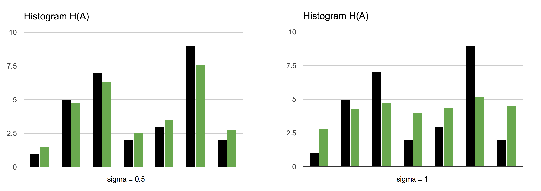
\includegraphics[width=450]{images/sigma_difference.pdf}
\caption{In green the smoothed version of the histogram in black, for two different values of the $\sigma$ parameter}
\label{fig:sigma_difference}
\end{figure}

In figure \ref{fig:smoothed_a_b} we can see the two histograms along with their smoothed version at $\sigma = 0.5$. The final distance will be the euclidean distance between the smoothed version. These are the distances at different smoothing levels:
\begin{align}
  \sigma = 0.5, \text{distance} = 6.91\nonumber\\
  \sigma = 1, \text{distance} = 6.09\nonumber\\
  \sigma = 2, \text{distance} = 5.53\nonumber
\end{align}
Without smoothing the distance would have been $7.74$, higher than any of the other distances. This is because, thanks to smoothing, we can take into account the fact the similarity of values in close bins. For instance, take $H(A,1) = 1$ which became $H(A,1) = 0.4$ after smoothing, thanks to the presence of the bin next to it which had a value of $3$.

\begin{figure}[h]
\centering
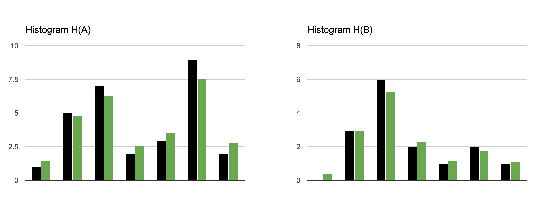
\includegraphics[width=450]{images/smoothed_a_b.pdf}
\caption{Original and smoothed versions of the two histograms $H(A)$ and $H(B)$ at $\sigma = 0.5$}
\label{fig:smoothed_a_b}
\end{figure}

